\documentclass[lang=cn,a4paper,newtx,bibend=bibtex]{elegantpaper}
\usepackage{env}
\title{Problems of Chapter 10.3.4-10.3.6}
\author{张志心 \ 计科2106}
\date{\zhdate{2024/04/23}}
\usepackage{env}
\pgfplotsset{compat=1.17}
\addbibresource[location=local]{reference.bib}
\begin{document}
\maketitle

\begin{prob}[Exercise 10.118]
  Prove Theorem 10.117 by induction.\\
  \textbf{Theorem 10.117~~} Let $\theta_n$ be the solution to the homogeneous
  linear difference equation
  \[
    \theta_{n+s} + \sum\limits_{i = 0}^{s - 1} \alpha_i \theta_{n+i} = 0.
  \]
  with constant coefficients $\alpha_i$'s and the initial values
  \[
    \MAT{\theta_0 & \theta_{-1} & \ddots & \theta_{-s+2} & \theta_{-s+1}}^T
    =
    \MAT{1 & 0 & \ddots & 0 & 0}^T.
  \]
  Then the inhomogeneous equation
  \[
    y_{n+s} + \sum\limits_{i = 0}^{s - 1} \alpha_{i} y_{n+i} = \psi_{n+s}
  \]
  with initial values $y_0, y_1, \cdots, y_{s-1}$ is uniquely solved by
  \[
    y_n = \sum\limits_{i=0}^{s-1}\theta_{n-i} \wanwan{y_i} + \sum\limits_{i=s}^n \theta_{n-i} \psi_i
  \]
  where 
  \[
    \MAT{\wanwan{y}_{s-1} \\ \wanwan{y}_{s-2} \\ \wanwan{y}_{s-3} \\ \ddots \\ \wanwan{y}_{1} \\ \wanwan{y}_0}
    =
    \MAT{
      1 & \theta_1 & \theta_2 & \cdots & \theta_{s-2} & \theta_{s-1} \\
      0 & 1 & \theta_1 & \cdots & \theta_{s-3} & \theta_{s-2} \\
      0 & 1 & 1 & \cdots & \theta_{s-3} & \theta_{s-2} \\
      \ddots & \ddots & \ddots & & \ddots & \ddots \\
      0 & 0 & 0 & \cdots & 1 & \theta_1 \\
      0 & 0 & 0 & \cdots & 0 & 1
    }^{-1} 
    \MAT{
      y_{s-1} \\ y_{s-2} \\ y_{s-3} \\ \ddots \\ y_1 \\ y_0
    }
  \]
\end{prob}

\begin{proof}
  当 $n \le s$ 时,结论显然成立。
  下面设结论对 $n = s+1, s+2, \cdots, n+s-1$ 均成立,则
  \equ{
    y_{n+s} &= -\sum\limits_{j=0}^{s-1} \alpha_i y_{n+i} + \psi_{n+s} \\
            &= -\sum\limits_{i=0}^{s-1} \alpha_i \left(\sum\limits_{j=0}^{s-1} \theta_{n+i-j} \wanwan{y}_j + \sum\limits_{j=s}^{n+i} \theta_{n+i-j} \psi_j\right) + \psi_{n+s} \\
            &= \sum\limits_{j=0}^{s-1} \theta_{n-j} \wanwan{y}_j + \sum\limits_{j=s}^{n+s-1} \theta_{n-j}\psi_j + \psi_{n+s} \\
            &= \sum\limits_{j=0}^{s-1} \theta_{n-j} \wanwan{y}_j + \sum\limits_{j=s}^{n+s} \theta_{n-j} \psi_j.
  }
\end{proof}


\begin{prob}[Exercise 10.123]
  Prove Lemma 10.122 by the approach similar with that for 
  Lemma 10.120, i.e., by considering the particular IVP Problems
  \equ{
    &u'(t) = f(t) = 0, u(0) = 1; \\
    &u'(t) = f(t) = 1, u(0) = 0.
  }
  \textbf{Lemma 10.122~~} A convergent LMM is consistent.
\end{prob}

\begin{proof}
  对 IVP \(u'(t) = 0, u(0) = 1\),由收敛性,\[\forall T > 0, \lim_{k \to 0, Nk = T} u^N = \lim_{k \to 0, Nk = T} \frac{1}{\alpha_s} \sum\limits_{j = 0}^{s-1} -\alpha_j u^{N-s+j} = 1.\]
  所以 \(\frac{1}{\alpha_s} \sum\limits_{j = 0}^{s-1} -\alpha_j = 1, \sum\limits_{j = 0}^s \alpha_j = 1\).
  对 IVP \(u'(t) = 1, u(0) = 0\),由收敛性,\[\forall T > 0, \lim_{k \to 0, Nk = T} u^N = \frac{1}{\alpha_s} \left(-\sum\limits_{j=0}^{s-1} \alpha_j u^{N-s+j} + k\sum\limits_{j=0}^s \beta_j \right) = T.\]\\
  所以 $\frac{1}{\alpha_s} \left(-\sum\limits_{j=0}^{s-1} \alpha_j k (N-s + j) + k\sum\limits_{j=0}^s \beta_j\right) = kN $. \\
  所以 $k\sum\limits_{j=0}^s \alpha_j (N-s+j) = k\sum\limits_{j=0}^s \beta_j \Rightarrow \sum\limits_{j=0}^s \alpha_j (N-s) + \sum\limits_{j=0}^s j\alpha_j = \sum\limits_{j=0}^s \beta_j$,\\
  因为 $\sum\limits_{j=0}^s \alpha_j =0$,所以 $\sum\limits_{j=0}^s j\alpha_j = \sum\limits_{j=0}^s \beta_j$。
\end{proof}


\begin{prob}[Exercise 10.138]
  Write a program to reproduce the RAS plots in Figures 10.4
  and 10.5.
\end{prob}

\begin{solution}~~\\
使用 python 绘制,代码如下:
\begin{verbatim}
import matplotlib.pyplot as plt 
import numpy as np 
import math as m 

def PLOT(f, leg, l=None, r=None, u = None, d = None, st = '-'):
  t = np.linspace(0, 2*m.pi, 5000)
  z = np.exp(1j*t)
  c = f(z)
  if(l != None):
      plt.xlim(left = l, right = r)
  if(u != None):
      plt.ylim(d, u)
  plt.plot(c.real, c.imag, linewidth = 0.7, color = 'black', label= leg, linestyle = st)
  plt.legend()
  
def bashforth1(z):
  return z-1
def bashforth2(z):
    return z*(z-1)/(3/2*z-1/2)
def bashforth3(z):
    return z*z*(z-1)/(23/12*z*z-16/12*z+5/12)
def bashforth4(z):
    return z*z*z*(z-1)/((55*z**3-59*z**2+37*z-9)/24) 

plt.figure(figsize=(6, 5))
PLOT(bashforth1, "p=1", -2.1, 0.1, -1.1, 1.1, st = ':')
PLOT(bashforth2, "p=2", st= "--")
PLOT(bashforth3, "p=3")
plt.show()
plt.figure(figsize=(6, 5))
PLOT(bashforth4, "p=4", -1.1, 1.1, -1.1, 1.1)
plt.show()

def moulton3(z):
    return z*(z-1)/(5*z**2+8*z-1)*12
def moulton4(z):
    return z*z*(z-1)/(9*z**3+19*z**2-5*z+1)*24
def moulton5(z):
    return z*z*z*(z-1)/(251*z**4+646*z**3-264*z**2+106*z-19)*720

plt.figure(figsize=(6, 5))
PLOT(moulton3, "p=3", -7, 1, -3.5, 3.5,st  = ":")
PLOT(moulton4, "p=4", st = "--")
PLOT(moulton5, "p=5")
plt.show()

def backward1(z):
    return (z-1)/z
def backward2(z):
    return (3*z**2-4*z+1)/(2*z**2)
def backward3(z):
    return (11*z**3-18*z**2+9*z-2)/(6*z**3)
def backward4(z):
    return (25*z**4-48*z**3+36*z**2-16*z+3)/(12*z**4)

plt.figure(figsize=(6, 5))
PLOT(backward1, "p=1", -4, 13, -7, 7, st = ":")
PLOT(backward2, "p=2", st = "--")
PLOT(backward3, "p=3", st= "-.")
PLOT(backward4, "p=4")
plt.show()
\end{verbatim}
\end{solution}

\begin{figure}[H]
  \centering
  \begin{subfigure}[b]{0.45\textwidth}
      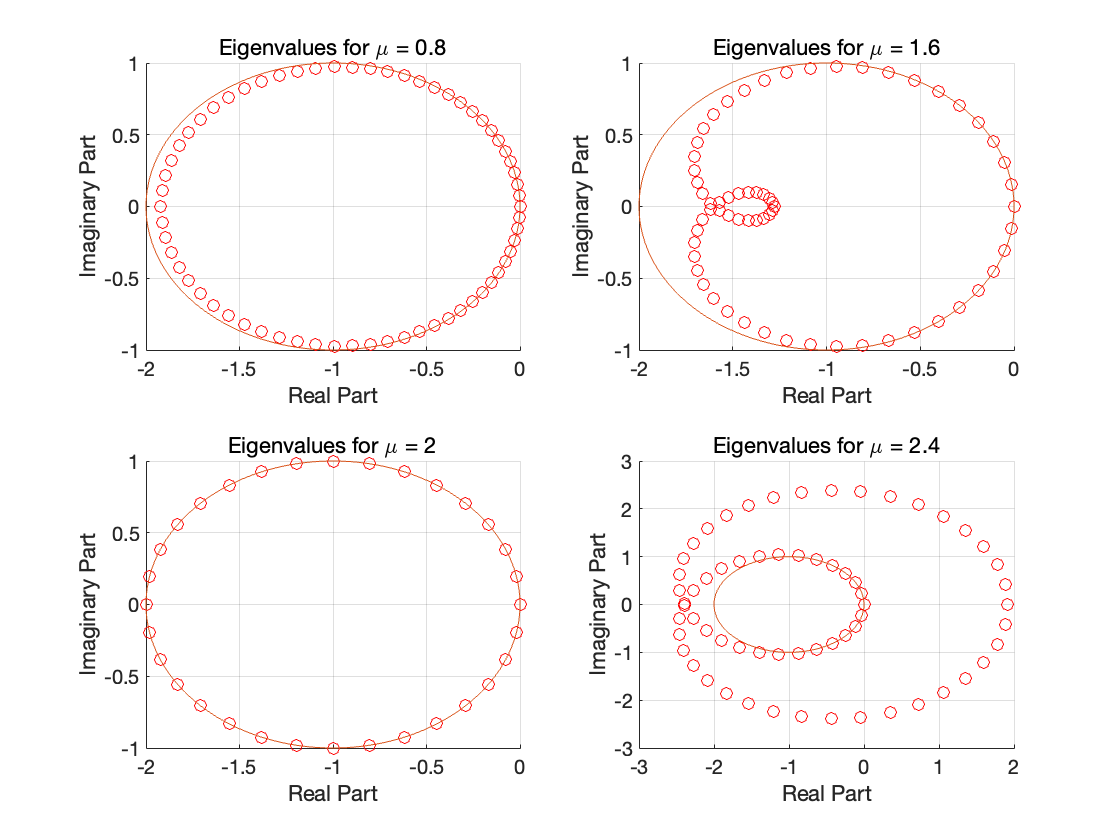
\includegraphics[width=\textwidth]{1.png}
  \end{subfigure}
  \hfill
  \begin{subfigure}[b]{0.45\textwidth}
      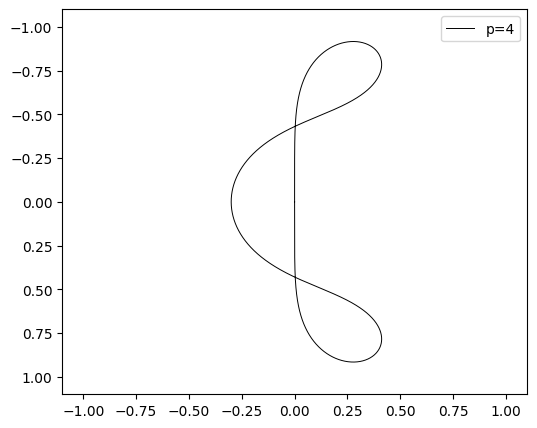
\includegraphics[width=\textwidth]{2.png}
  \end{subfigure}
  \caption{The bounded RAS of Adams-Bashforth formu-
  las for $p = 1, 2, 3$ (left) and $p = 4$ (right).}
\end{figure}

\begin{figure}[H]
  \centering
  \begin{subfigure}[b]{0.45\textwidth}
      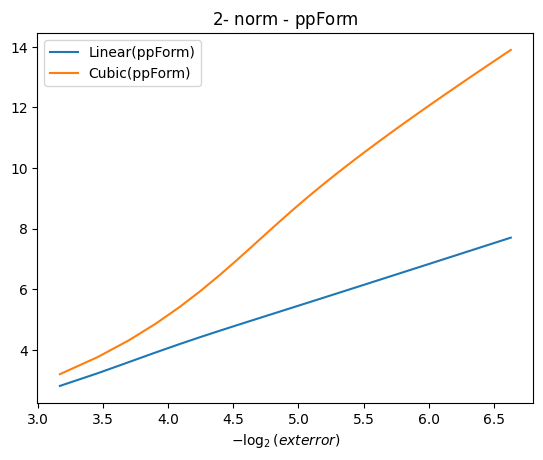
\includegraphics[width=\textwidth]{3.png}
  \end{subfigure}
  \hfill
  \begin{subfigure}[b]{0.45\textwidth}
      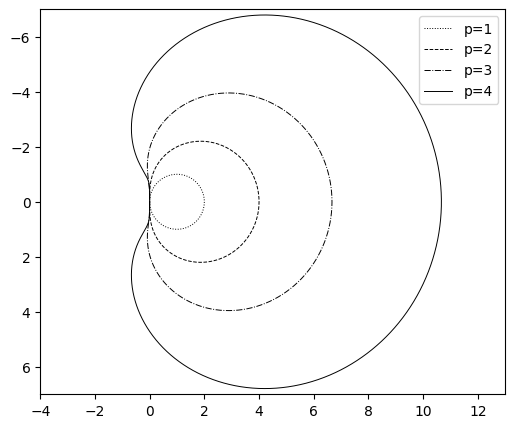
\includegraphics[width=\textwidth]{4.png}
  \end{subfigure}
  \caption{The bounded RASs of Adams-Moulton for-
  mulas with $p = 3, 4, 5$ (left) and the unbounded RASs of
  backward differentiation formulas with $p = 1, 2, 3, 4$ (right)}
\end{figure}


\nocite{*}
\printbibliography[heading=bibintoc, title=\ebibname]
\end{document}